\documentclass{novel}
\usepackage{wrapfig}
\usepackage{lettrine}
\usepackage{pdfpages}
\usepackage{changepage}

\lang      {english}
\title     {}
\subtitle  {}
\authors   {}
\cover     {resources/novel_front.jpg}{resources/novel_back.jpg}
\license   {CC}{by-nc-sa}{4.0}
\isbn      {ECS661U}
\publisher {210517307 \& 210543960}
\edition   {1}{2024}
\dedicate  {Queen Mary University of London}{User Experience Design}
\thank     {Coursework 1}
\keywords  {fiction, template, packages}

\note{This report explores the relationship between technology and London's libraries. As the modern world of computers and smartphones intertwine with the traditional practise of reading, our findings are aptly presented in the classic format of a book.}

\blurb{"Technology in England’s Libraries" explores the effects of devices on user experience. This ethnographic study examines how technology and noise levels affect one another, with data taken from the historic British Library to the modest Lewsey Library. By observing real-world interactions, our research reveals how technology influences learning, social interaction, and personal comfort. \\ \\ Furthermore, this book proposes an innovative new design, created to enhance the library experience through auditory, visual, and tactile feedback to promote quiet and respectful spaces without imposing on visitors or sacrificing collaborative opportunity.}

\begin{document}

\toc

\h{Introduction}
\l{T}his ethnographic study focuses on the dynamics and user behaviours within different library environments, examining their contribution to the user experience. Libraries, as essential resources for learning and research, provide spaces that significantly affect users' productivity and comfort levels. The aim of this research is to understand how various elements within library settings, such as room size, noise levels, and technology use, interact to create distinct user experiences.

The study was conducted in five different libraries: the British Library Membership Room, Whitechapel Library, Mile End Library, Bethnal Green Library, and Lewsey Library. These libraries were selected for their varied sizes and the diverse communities they serve. Each location was observed once, providing a snapshot of typical user behaviour and environment interaction at different times.

By examining the interplay between space, noise, and technology use, we can gain a better understanding of the ideal conditions for different types of library users and how libraries can adapt to meet their users' needs more effectively.

\noindent
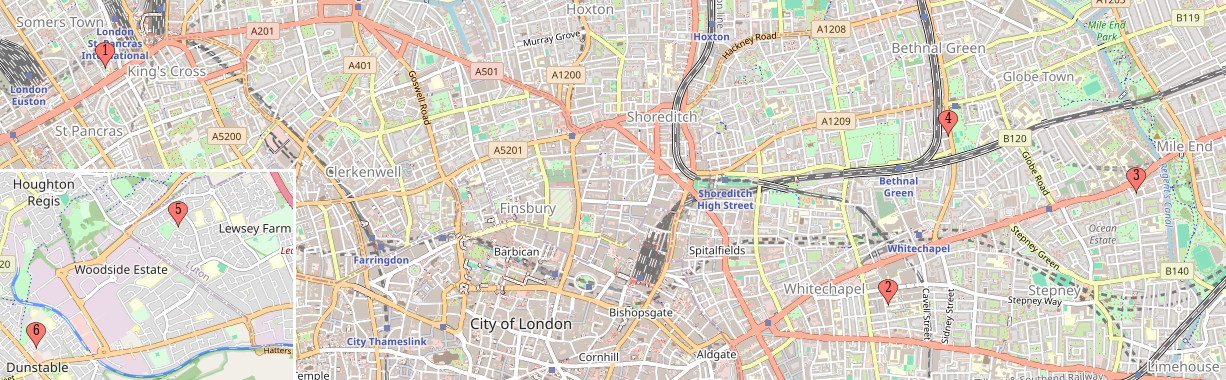
\includegraphics[width=\textwidth]{resources/Map2.png}

\h{Observations}


\l{M}ile End Library presents a scenario where technology facilitates social interaction and a sense of community among students. However, this comes at the cost of individual concentration and quiet study. Here, laptop usage was notably higher. In one scenario, a group of four students sharing their exam results led to periods of raised voices and laughter. This interaction highlights how technology can distract people from their surroundings. While for some, this behaviour may create memorable moments that alleviate academic pressure and encourage friendships and communal learning, for others, it may distract from urgent work and increase stress.

\begin{wrapfigure}{r}{0.3\textwidth} 
    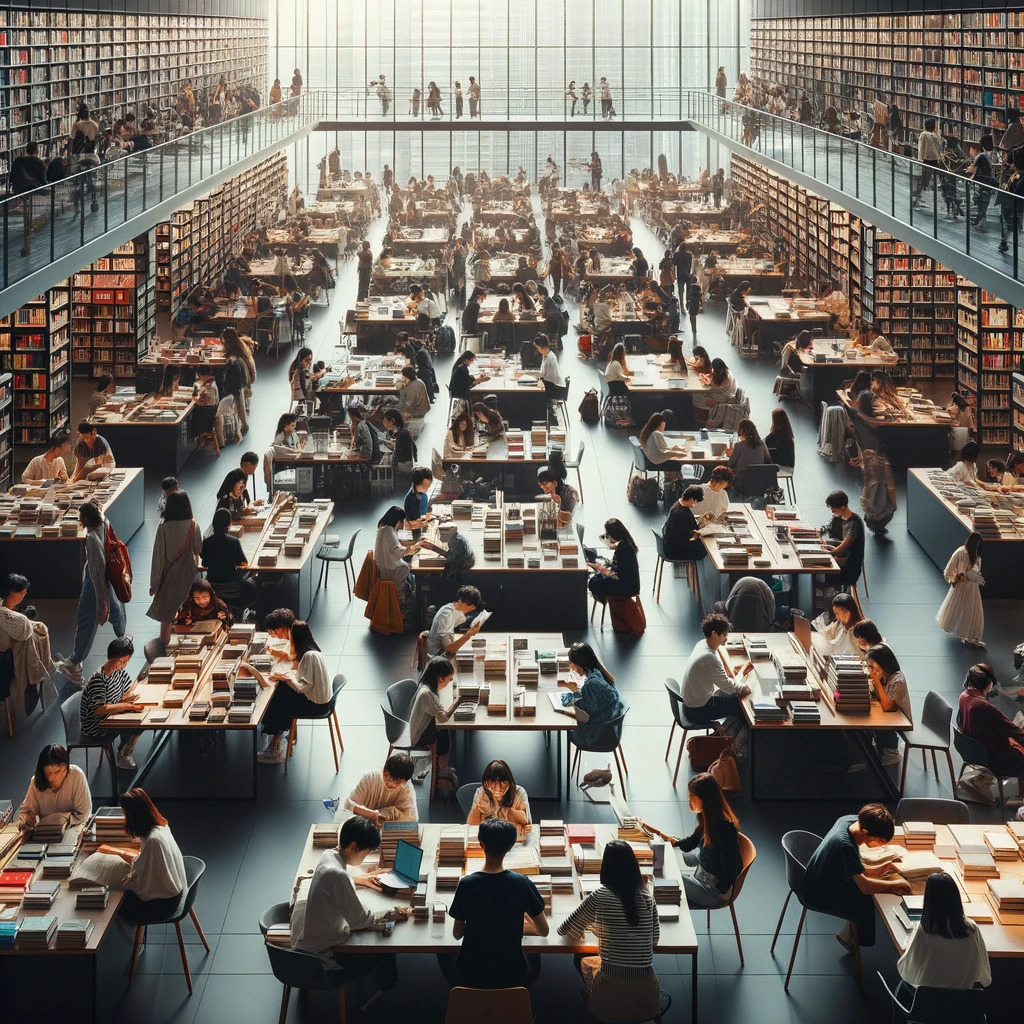
\includegraphics[width=0.3\textwidth]{resources/mileEnd.jpg}
\end{wrapfigure}

Unfortunately, for those seeking a quieter space, silent areas are not a significant improvement. In the Mile End Library's quiet area, three individuals, focused on their laptops, were observed discussing a group project. Shared content on their screens led them to gradually escalate beyond whispering levels. This breach of quiet room etiquette was not due to malice but rather to the nature of their collaborative work and the insulating effect of laptop screens, which can create a false sense of privacy. This incident presents the challenge of maintaining silence in spaces where technology encourages collaboration and communication.

The British Library Membership Room and the Whitechapel Library, both classified as small rooms, exhibited different levels of vocal interaction. While the British Library had four individuals engaging in conversation, the Whitechapel Library had no vocal interactions. This variation is likely due to architectural design; Whitechapel Library's tall ceiling reduces echo, encouraging visitors to maintain silence. Conversely, the Mile End Library, with a very large room size, had significant amounts of loud and moderate conversations, likely due to the perception of anonymity in larger spaces and the less direct impact of noise on immediate surroundings. Since both libraries are almost entirely composed of students, it appears that categories of people are not the sole determinant of noise levels.

\begin{wrapfigure}{l}{0.3\textwidth} 
\vspace{-\intextsep}
    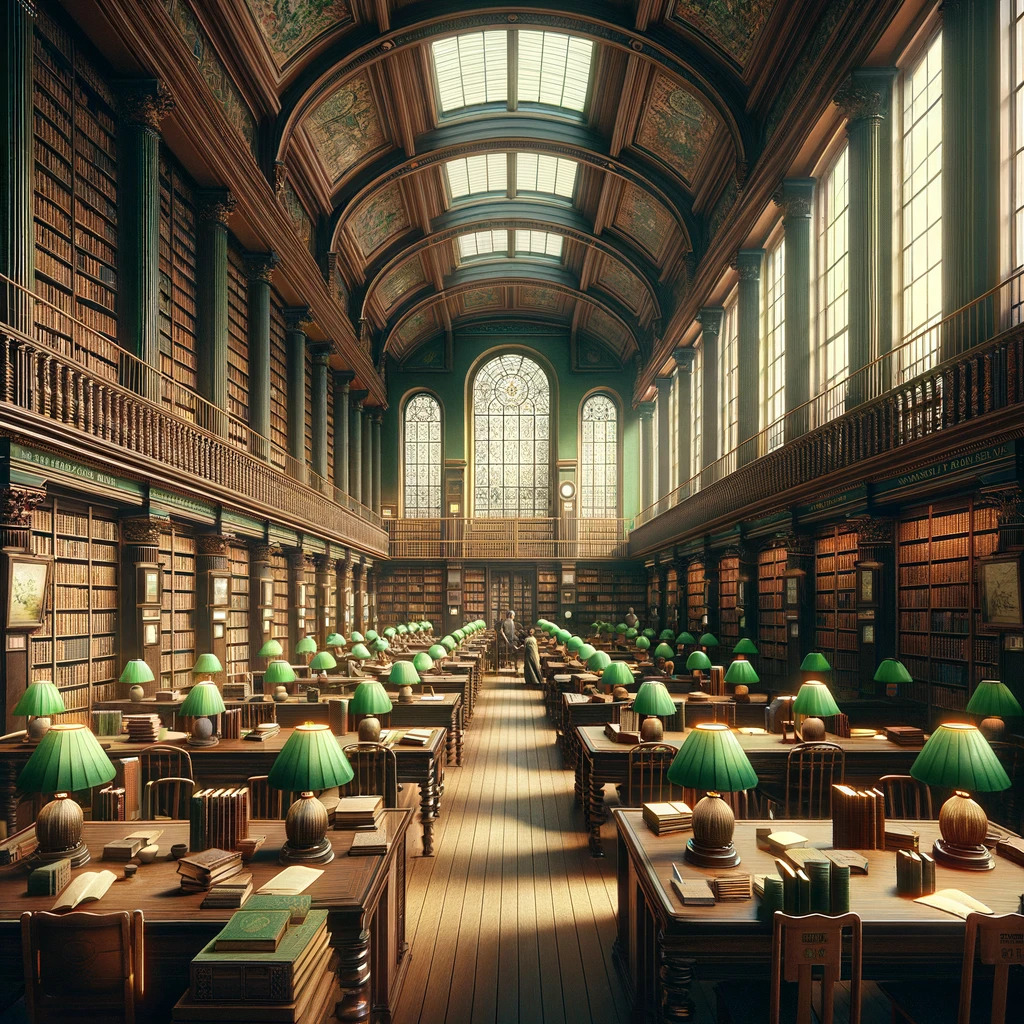
\includegraphics[width=0.3\textwidth]{resources/whitechapel.jpg}
    \vspace{-50pt} % Adjust this value as needed to reduce the gap below the image
\end{wrapfigure}
At the Whitechapel Library, despite a notable number of individuals on mobile phones, the environment remained quiet. This indicates respectful phone usage that does not disturb others. This behaviour reflects community adherence to silent norms, influenced by the library's architectural design, which discourages loud speaking. The Lewsey Library had no reported phone usage, yet two people were talking loudly. This suggests that technology is not the only factor influencing noise; social dynamics and library policies (or their enforcement) also play significant roles.

\begin{wrapfigure}{r}{0.3\textwidth} 
    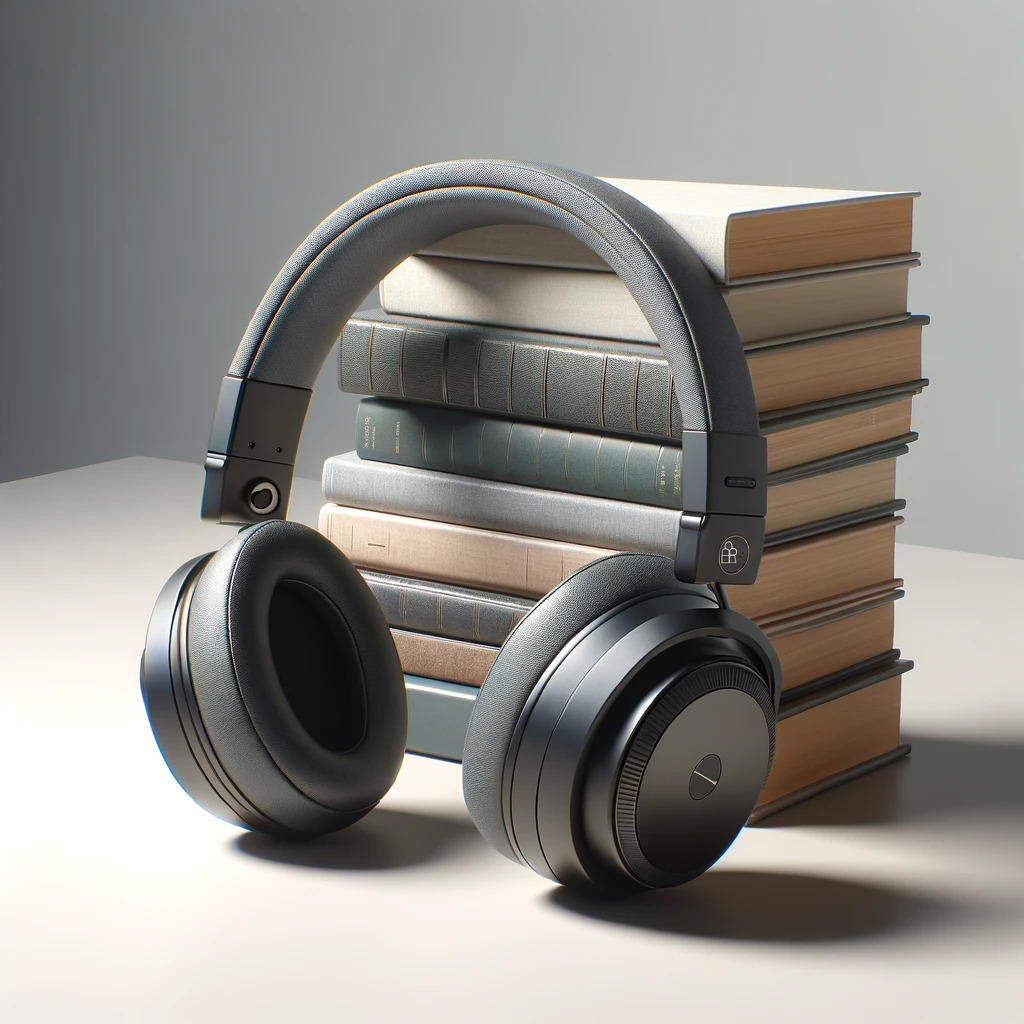
\includegraphics[width=0.3\textwidth]{resources/headphones.jpg}
\end{wrapfigure}
In Bethnal Green Library and Whitechapel library, the advent of noise-cancelling headphones represents a significant move towards private space within a public setting. Most individuals were immersed in their own worlds, undisturbed by their surroundings. This technology enables users to create a 'private bubble,' isolating themselves from potential distractions and transforming a segment of the library into a personal study area. In these cases, technology seems to improve noise levels, especially since the receptionist at Bethnal Green, a small library where every pin drop can be heard, had a prolonged conversation with a visitor.

The presence of technology does not inherently increase noise; instead, it is the type of technology use and the social context that dictate the sound level. Individuals using laptops with headphones contribute to a quiet environment, whereas groups using technology for collaborative work may increase overall noise. The wide range of factors contributing to noise levels in a library requires a universal solution to the issue.

Despite the widespread availability of e-books, digital archives, and online databases, libraries continue to hold a significant place in communities for several reasons. While their access to social interaction and collaboration should not be underplayed, their history as safe, quiet, inclusive spaces must be protected.

\h{Design}
\l{T}he system will integrate auditory, visual, and tactile feedback mechanisms. For example, when noise levels exceed a certain threshold, the system could emit a gentle, non-intrusive sound reminder, while the visual display changes colours. Tactile feedback could be provided through library desks that have integrated vibration alerts, subtle enough to catch attention without causing disturbance. This multi-modal approach ensures that the system accommodates different learning and interaction preferences, drawing from the Universal Design principles (Connell et al., 1997). This not only accommodates various sensory preferences and needs, but also gives the system multiple routes by which to catch the attention of overly loud visitors. This approach ensures that all users, including those with disabilities, can receive and understand noise level information, thus fostering an environment that encourages everyone to control and be conscious of the ambient noise around them.

\noindent
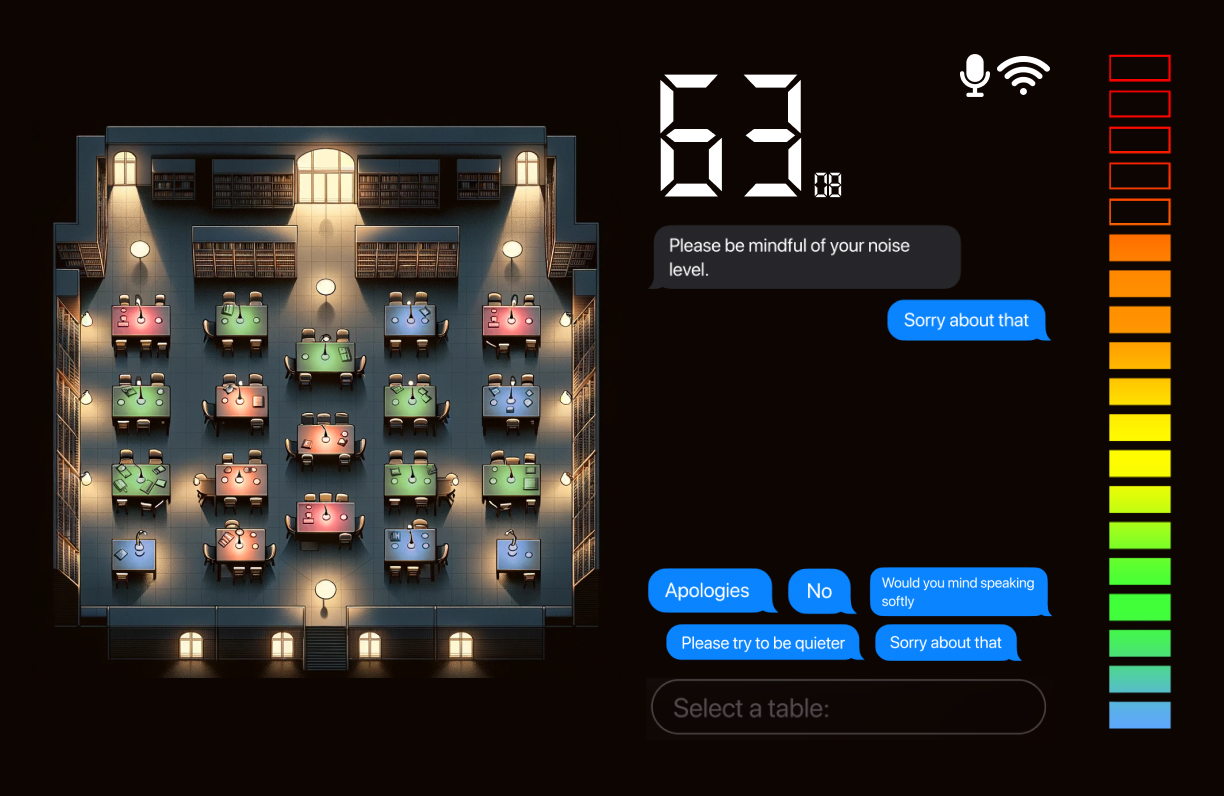
\includegraphics[width=\textwidth]{resources/design.jpg}

The system promotes a collective responsibility towards maintaining a conducive work environment. Inspired by theories of social proof (Cialdini, 2001), when individuals observe others modifying their behaviour based on the displayed noise levels, they are likely to follow suit. By including an algorithm to alert users that they are much louder than the average desk, we can pressure outliers to reduce their noise levels to decrease distractions for others. Together with giving users the ability to send polite, anonymous messages to nearby desks, we can foster a social governance model. Users collectively contribute to the maintenance of an efficiency and peaceful environment. This approach is supported by the theory of social translucence by Erickson and Kellogg (2000), which advocates for systems that support cooperative behaviours through social cues. In a worst case scenario where noise is significantly above a predetermined level, staff or security can be notified to visit or view the desk on cctv. This will increase safety in libraries, and users that are aware of this feature can use it to call for help in emergencies.

\begin{wrapfigure}{r}{0.3\textwidth}
\vspace{-\intextsep}
    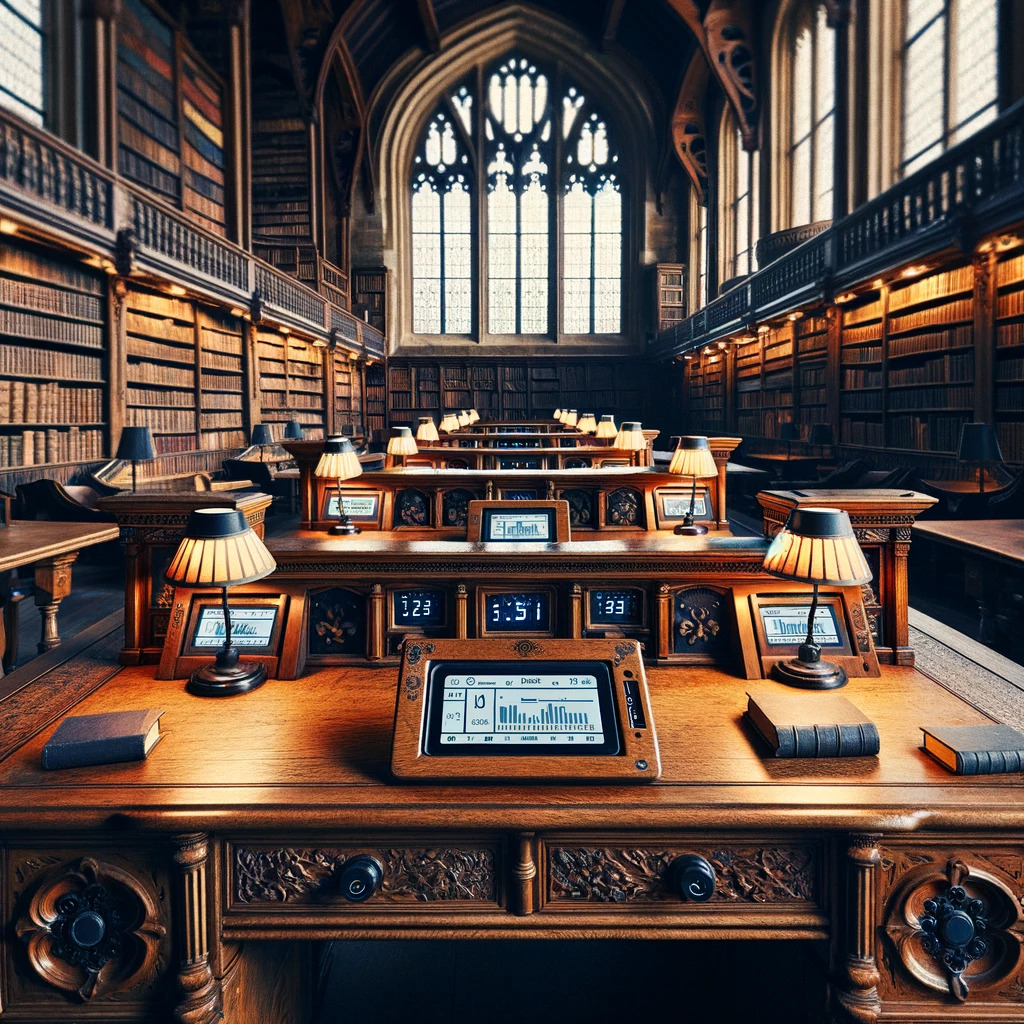
\includegraphics[width=0.3\textwidth]{resources/deskDevice.jpg}
    \vspace{-20pt} % Adjust this value as needed to reduce the gap below the image
\end{wrapfigure}
The display will not only serve a functional purpose but also contribute to the library's ambiance. Drawing on principles from calm technology (Weiser and Brown, 1996), the design will be unobtrusive, blending with the library's aesthetic by integrating small screens into desks. Colors and patterns will be chosen based on research in color psychology (Elliot et al., 2007), with pastel blue and green colors representing acceptable noise levels and bright red colors indicating higher noise levels. A default dark mode in the UI will reduce the light pollution in the library, decibel counters will appear as a segmented display, and it, along with all other ui elements will only update once a second, to match that of a clock to avoid distractions.

Noise level data is processed locally without recording specific sounds or conversations, and communication between desks is anonymized. Respecting user privacy is crucial in fostering trust and acceptance of interactive systems. By ensuring data is processed locally and interactions remain anonymous, ALD adheres to the privacy-by-design principles outlined by Cavoukian (2009). In any case, a microphone indicator will always be shown on the display to alert users that their voices are being captured.

ALD allowed libraries to provide virtual leaves for maintaining a quiet environment. These can be exchanged for real-world rewards, leveraging the psychological impact of rewards and aligning with the principles of motivational design (Deterding et al., 2011). For libraries without the financial capabilities, the display can instead feature showing a tranquil forest that becomes more animated as noise levels decrease. This provides a subtle distraction that encourages noise reduction without breaking concentration, while promoting noise control in a positive and motivating way.

\h{Data}
\begin{adjustwidth}{-2cm}{-2cm}
    \centering
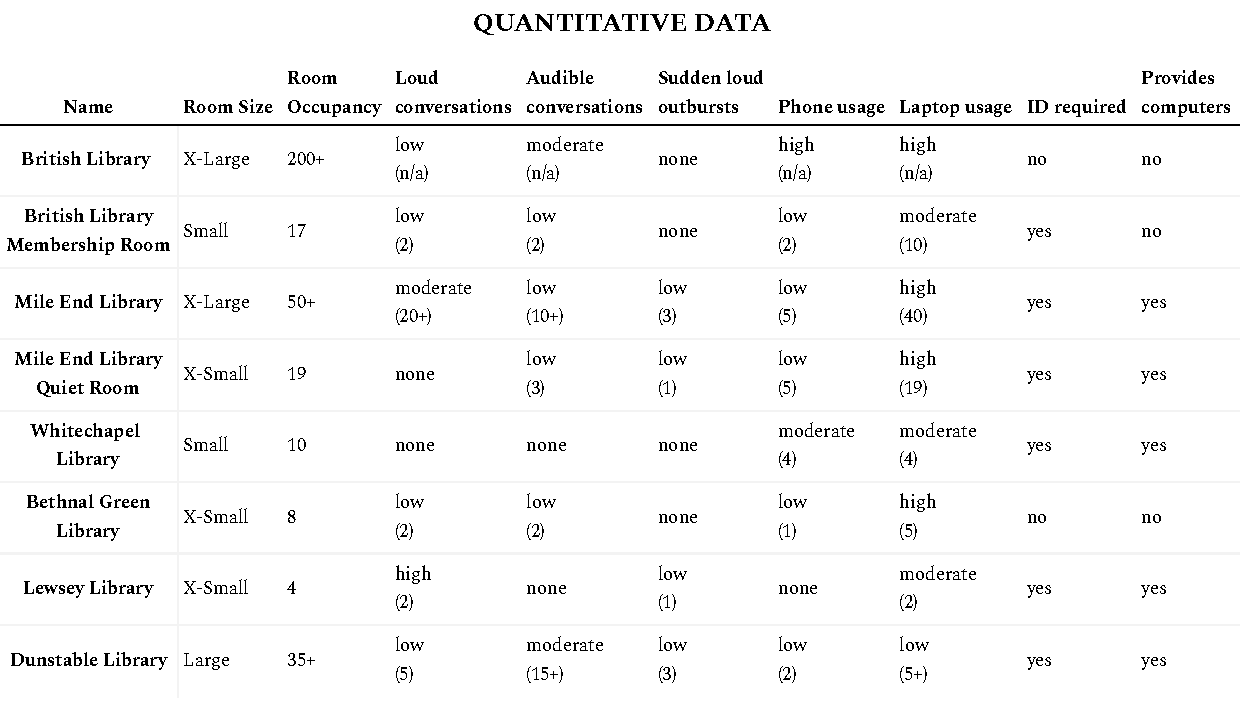
\includegraphics[width=\dimexpr\paperwidth-4cm\relax]{resources/nData.pdf}
\end{adjustwidth}

\begin{adjustwidth}{-2cm}{-2cm}
    \centering
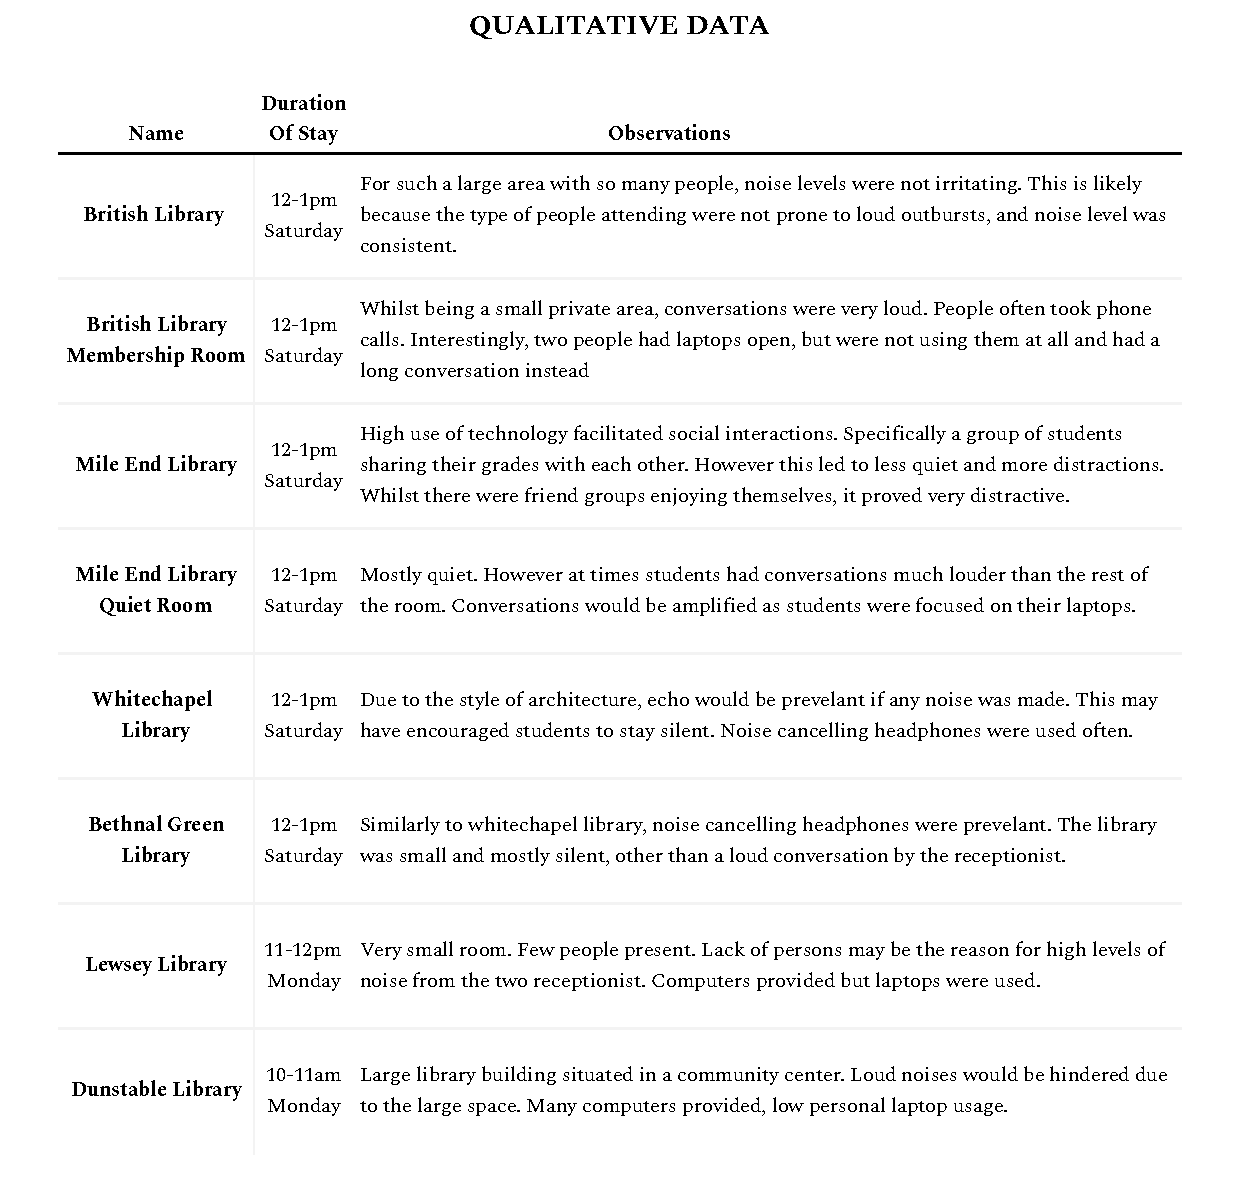
\includegraphics[width=\dimexpr\paperwidth-4cm\relax]{resources/lData.pdf}
\end{adjustwidth}

\h{References}

\end{document}
